\documentclass[xcolor=pdflatex,dvipsnames,table]{beamer}
\usepackage{epsfig,graphicx}
\usepackage{palatino}
\usepackage{fancybox}
\usepackage{relsize}
\usepackage[procnames]{listings}
\usepackage{hyperref}
\usepackage{qtree} % needed?
\usepackage{booktabs}
\usepackage{dirtree}
\usepackage[normalem]{ulem}


% fatter TT font
\renewcommand*\ttdefault{txtt}
% another TT, suggested by Alex
% \usepackage{inconsolata}
% \usepackage[T1]{fontenc} % needed as well?


\newcommand{\scale}{0.7}

\newcommand{\todo}[1]{{\emph{TODO: #1}}}
\newcommand{\martin}[1]{{\color{blue} Martin: #1}}
\newcommand{\abcdef}[1]{{\color{red} Author2: #1}}

% uncomment following for final submission
%\renewcommand{\todo}[1]{}
%\renewcommand{\martin}[1]{}
%\renewcommand{\author2}[1]{}

\newcommand{\code}[1]{{\texttt{#1}}}

\hypersetup{
  linkcolor  = black,
%  citecolor  = blue,
  urlcolor   = blue,
  colorlinks = true,
}

\beamertemplatenavigationsymbolsempty
\setbeamertemplate{footline}[frame number]





\newif\ifbook
% shared in slides and book

\lstdefinelanguage{chisel}{
  morekeywords={abstract,case,catch,class,def,%
    do,else,extends,false,final,finally,%
    for,if,implicit,import,match,mixin,%
    new,null,object,override,package,%
    private,protected,requires,return,sealed,%
    super,this,throw,trait,true,try,%
    type,val,var,while,with,yield},
  otherkeywords={=>,<-,<\%,<:,>:,\#,@},
  sensitive=true,
  morecomment=[l]{//},
  morecomment=[n]{/*}{*/},
  morestring=[b]",
  morestring=[b]',
  morestring=[b]"""
}

\usepackage{color}
\definecolor{dkgreen}{rgb}{0,0.6,0}
\definecolor{gray}{rgb}{0.5,0.5,0.5}
\definecolor{mauve}{rgb}{0.58,0,0.82}

% Default settings for code listings
\ifbook
\lstset{%frame=lines,
  language=chisel,
  aboveskip=3mm,
  belowskip=3mm,
  showstringspaces=false,
  columns=fixed, % basewidth=\mybasewidth,
  basicstyle={\small\ttfamily},
  numbers=none,
  numberstyle=\footnotesize,
  % identifierstyle=\color{red},
  breaklines=true,
  breakatwhitespace=true,
  procnamekeys={def, val, var, class, trait, object, extends},
  % procnamestyle=\ttfamily,
  tabsize=2,
  float
}
\else
\lstset{%frame=lines,
  language=chisel,
  aboveskip=3mm,
  belowskip=3mm,
  showstringspaces=false,
  columns=fixed, % basewidth=\mybasewidth,
  basicstyle={\small\ttfamily},
  numbers=none,
  numberstyle=\footnotesize\color{gray},
  % identifierstyle=\color{red},
  keywordstyle=\color{blue},
  commentstyle=\color{dkgreen},
  stringstyle=\color{mauve},
  breaklines=true,
  breakatwhitespace=true,
  procnamekeys={def, val, var, class, trait, object, extends},
  procnamestyle=\ttfamily\color{red},
  tabsize=2,
  float
}
\fi

\lstnewenvironment{chisel}[1][]
{\lstset{language=chisel,#1}}
{}

\newcommand{\shortlist}[1]{{\lstinputlisting[nolol]{#1}}}

\newcommand{\longlist}[3]{{\lstinputlisting[float, caption={#2}, label={#3}, frame=tb, captionpos=b]{#1}}}

\newcommand{\verylonglist}[3]{{\lstinputlisting[caption={#2}, label={#3}, frame=tb, captionpos=b]{#1}}}


\title{Verification of Digital Designs: Introduction}
\author{Martin Schoeberl}
\date{\today}
\institute{Technical University of Denmark\\
Embedded Systems Engineering}

\begin{document}

\begin{frame}
\titlepage
\end{frame}


\begin{frame}[fragile]{Overview}
\begin{itemize}
\item Motivation
\item Course organization
\item Languages for digital hardware design
%\item Testing (see 2.1.4)
\item Debugging, Testing, and Verification
\item A little bit of Scala
\item An Exercise
\end{itemize}
\end{frame}


\begin{frame}[fragile]{Motivation}
\begin{itemize}
\item We had a meeting with DK industry in June
\item Missing design verification
\item For one developer there are 2--3 verification engineers
\item Testing is considered boring, but it does not have to be
\item Best is to be a developer and a verification engineer
\item Change roles, we will do in this course
\end{itemize}
\end{frame}

\begin{frame}[fragile]{Course Organization}
\begin{itemize}
\item This is a special course
\item Not just me giving talks and preparing exercises
\begin{itemize}
\item But I will bring in some
\item You will bring in some as well
\end{itemize}
\item This is a lot about self study
\item You will bring up material
\item We will use GitHub for material, exercises, project
\begin{itemize}
\item Slides are there as well
\item \url{https://github.com/chisel-uvm/class2020}
\item Let's signup right now ;-)
\end{itemize}
\end{itemize}
\end{frame}

\begin{frame}[fragile]{Technicalities}
\begin{itemize}
\item We will use Chisel/Scala for tesing
\item VHDL, SystemVerilog, UVM are optional
\item You need to setup your laptop
\begin{itemize}
\item see: https://github.com/schoeberl/chisel-lab/blob/master/Setup.md
\item We will not use an FPGA
\end{itemize}
\item abc
\item abc
\item abc
\item abc
\item abc
\end{itemize}
\end{frame}

\begin{frame}[fragile]{Reading Material}
\begin{itemize}
\item No \emph{good} book on DV
\item We need to find
\begin{itemize}
\item Web sites
\item Blogs
\item Articles (popular, e.g., EE Times)
\item Paper (conferences)
\item Look what software people do
\item ...
\end{itemize}
\item Your homework: search literature till next week
\item Present what you found
\end{itemize}
\end{frame}

\begin{frame}[fragile]{Title}
\begin{itemize}
\item abc
\item abc
\item abc
\item abc
\item abc
\item abc
\item abc
\item abc
\item abc
\end{itemize}
\end{frame}



\begin{frame}[fragile]{This is an Open-Access/Open-Source Course}
\begin{itemize}
\item Almost all material is public visible
\item Slides are open access
\item Lab material is open access
\item Hosted on GitHub
\begin{itemize}
\item \textbf{You} can contribute with a pull request
\item Becoming an author of this course :-)
\end{itemize}
\item The Chisel book is freely available
\end{itemize}
\end{frame}



\begin{frame}[fragile]{Chisel Overview}
\begin{itemize}
\item A hardware \emph{construction} language
\begin{itemize}
\item Constructing Hardware In a Scala Embedded Language
\item If it compiles, it is synthesisable hardware 
\item Say goodby to your unintended latches
\end{itemize}
\item Chisel is not a high-level synthesis language
\item Single source for two targets
\begin{itemize}
\item Cycle accurate simulation (testing)
\item Verilog for synthesis
\end{itemize}
\item Embedded in Scala
\begin{itemize}
\item Full power of Scala available
\item But to start with, no Scala knowledge needed
\end{itemize}
\item Developed at UC Berkeley
\end{itemize}
\end{frame}

\begin{frame}[fragile]{Some Notes on Scala}
\begin{itemize}
\item Object oriented
\item Functional
\item Strongly typed
\begin{itemize}
\item With very good type inference
\end{itemize}
\item Could be seen as Java++
\item Compiled to the JVM
\item Good Java interoperability
\begin{itemize}
\item Many libraries available
\item You can write your testing code in Java
\end{itemize}
\end{itemize}
\end{frame}

\begin{frame}[fragile]{Chisel vs. Scala}
\begin{itemize}
\item A Chisel hardware description is a Scala program
\item Chisel is a Scala library
\item When the program is executed it generates hardware
\item Chisel is a so-called \emph{embedded domain-specific language}
\end{itemize}
\end{frame}


\begin{frame}[fragile]{Free Tools for Chisel and FPGA Design}
\begin{itemize}
\item \href{https://adoptopenjdk.net/}{Java OpenJDK 8} already installed for Java course
\item \href{https://www.scala-sbt.org/}{sbt, the Scala (and Java) build tool}
\item \href{https://www.jetbrains.com/idea/download/}{IntelliJ (the free Community version)}
\item \href{http://gtkwave.sourceforge.net/}{GTKWave}
\item \href{https://www.xilinx.com/products/design-tools/vivado/vivado-webpack.html}{Vivado WebPACK} already installed from DE1
% \item \href{http://www.altera.com/products/software/quartus-ii/web-edition/qts-we-index.html}{Quartus}
\item Nice to have:
\begin{itemize}
\item make, git
\end{itemize}
\end{itemize}
\end{frame}

\begin{frame}[fragile]{Tool Setup for Different OSs}
\begin{itemize}
\item Windows
\begin{itemize}
\item Use the installers from the websites
\end{itemize}
\item macOS
\begin{itemize}
\item \code{brew install sbt}
\item For the rest, use the installer from the websites
\end{itemize}
\item Linux/Ubuntu
\begin{itemize}
\item \code{sudo apt install openjdk-8-jdk git make gtkwave}
\item Install sbt, see \url{https://github.com/schoeberl/chisel-lab/blob/master/Setup.md}
\item IntelliJ as from the website
\end{itemize}
\end{itemize}
\end{frame}

\begin{frame}[fragile]{An IDE for Chisel}
\begin{itemize}
\item IntelliJ
\item Scala plugin
\item For IntelliJ: File - New - Project from Existing Sources..., open build.sbt
%\item But you are not compiling with Eclipse\\ and against the Chisel source
\item Show it (down to the Basys3)
\end{itemize}
\end{frame}


\begin{frame}[fragile]{A Chisel Book}
\begin{figure}
    \centering
    \href{https://github.com/schoeberl/chisel-book}{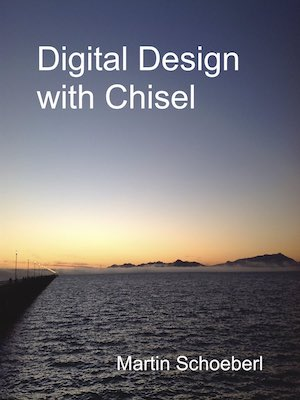
\includegraphics[scale=0.4]{../cover-small}}
\end{figure}

\begin{itemize}
\item Available in open access (as PDF)
\begin{itemize}
\item Optimized for reading on a tablet (size, hyper links)
\end{itemize}
\item Amazon can do the printout
\end{itemize}
\end{frame}

\begin{frame}[fragile]{Further Information}
\begin{itemize}
\item \url{https://www.chisel-lang.org/}
\item \url{https://github.com/freechipsproject/chisel-cheatsheet/releases/latest/download/chisel_cheatsheet.pdf}
\item \url{https://github.com/ucb-bar/chisel-tutorial}
\item \url{https://github.com/ucb-bar/generator-bootcamp}
%\item Chisel 2 documentation at \url{https://github.com/schoeberl/chisel2-doc}
%\begin{itemize}
%\item Chisel 2.2 Tutorial
%\item Getting Started with Chisel
%\end{itemize}
\item \url{http://groups.google.com/group/chisel-users}
\item \url{https://github.com/schoeberl/chisel-book}
\end{itemize}
\end{frame}


\begin{frame}[fragile]{Lab Time: Hello World Testing}
\begin{itemize}
\item xxx
\end{itemize}
\end{frame}



\begin{frame}[fragile]{Summary}
\begin{itemize}
\item xxx
\end{itemize}
\end{frame}

\end{document}

\begin{frame}[fragile]{Title}
\begin{itemize}
\item abc
\end{itemize}
\end{frame}
